\section{Results}
\label{sec:results}

\subsection{Damage under LoRA}
The balanced CE model reaches 36.53 percent BA $[33.82, 39.45]$. It loses $D=3.54$ points $[1.93, 5.21]$ at $\rho=50$ and $4.95$ points $[3.25, 6.74]$ at $\rho=100$. At native shares the damage is $0.85$ points $[-0.31, 2.08]$, an interval that includes zero. All three damages are smaller than under the frozen readout, which lost 6.63, 7.65, and 4.05 points on the same test patients \citep{queisler2026prevalenceBracs}. The reason is the undamaged reference, not the imbalanced allocations: LoRA's balanced model is about three points less accurate than the frozen readout (36.53 against 39.57 percent), while the imbalanced models land close to the frozen values (32.99 against 32.94 at $\rho=50$, 31.57 against 31.92 at $\rho=100$, 35.67 against 35.51 at N).

\subsection{Recovery per method}
Figure~\ref{fig:recovery} and Table~\ref{tab:recovery} give each method's paired recovery. At $\rho=100$, six of eight variants recover a material part of the damage: CUDA (2.59 points $[1.42, 3.79]$), train-time and post-hoc logit adjustment (1.96 and 1.94), classifier-only and end-to-end GCL (1.77 and 1.48), and balanced sampling (1.14). cRT (0.88) and DisAlign (0.58) recover a positive amount below the one-point threshold. CUDA's share of the damage, 0.52 $[0.29, 0.82]$, is the largest, followed by logit adjustment's 0.40 $[0.19, 0.60]$; no share interval reaches 1, so part of the damage remains under every method. CUDA alone formally reaches full recovery at $\rho=100$: the interval of its accuracy, $[31.70, 36.81]$, just contains the balanced 36.53 percent, while its paired share places the remaining gap between about one-fifth and seven-tenths of the damage.

At $\rho=50$ the ordering is the same with smaller gains. CUDA (1.81 points, share 0.51 $[0.20, 0.91]$), logit adjustment (both forms), and GCL (both forms) recover a material part, the latter four with shares of 0.31 to 0.41, and balanced sampling falls just short (0.72, interval includes zero). These five variants also formally reach full recovery, because the interval of an unpaired accuracy is about five points wide, wider than the 3.54-point damage; their paired shares, whose intervals end below 0.92, show that the gap is not closed. At native shares, seven of eight recoveries lie between $-0.17$ and $0.45$ points with an interval that includes zero. CUDA is the exception: it gains 1.21 points $[0.34, 2.14]$ and reaches 36.89 percent, above the balanced CE model's 36.53, although the damage it would recover, 0.85 points, cannot be distinguished from zero.

\begin{figure}[t]
  \centering
  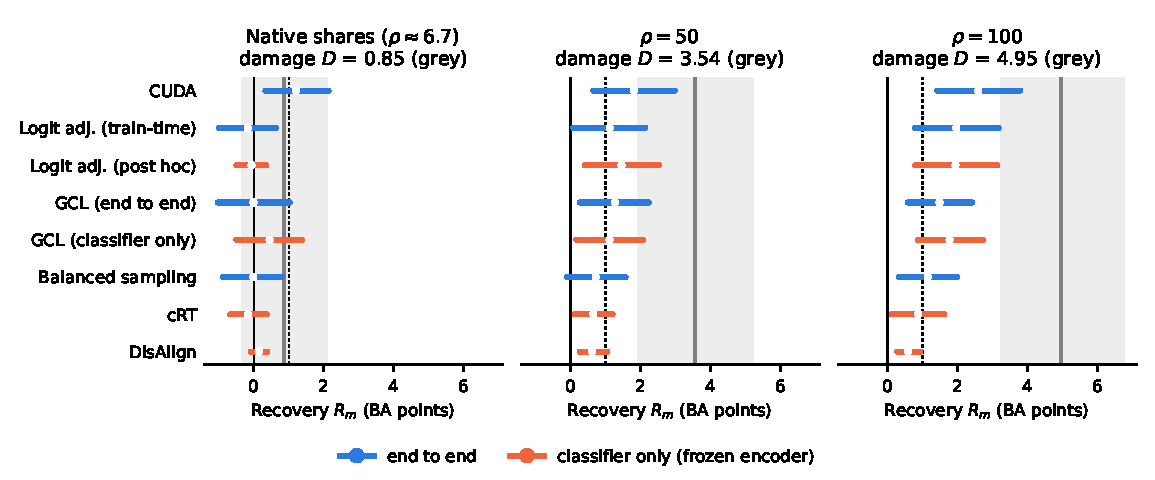
\includegraphics[width=\textwidth]{fig_recovery.pdf}
  \caption{CUDA, logit adjustment, and GCL recover one to three points at $\rho=50$ and $\rho=100$, short of the damage; at native shares only CUDA moves. Paired recovery $R_m$ with 95\% intervals. The grey line and band mark the CE damage $D$ with its interval, the solid line zero, and the dotted line the one-point threshold.}
  \label{fig:recovery}
\end{figure}

\begin{table}[t]
\centering
\footnotesize
\setlength{\tabcolsep}{3.5pt}
\resizebox{\textwidth}{!}{%
\begin{tabular}{@{}lccccc@{}}
\toprule
& \multicolumn{2}{c}{$\rho=50$ ($D=3.54$)} & \multicolumn{2}{c}{$\rho=100$ ($D=4.95$)} & N ($D=0.85$) \\
\cmidrule(lr){2-3}\cmidrule(lr){4-5}\cmidrule(lr){6-6}
Method & $R_m$ & share & $R_m$ & share & $R_m$ \\
\midrule
CUDA & \textbf{1.81} $[0.65, 2.97]$ & 0.51 $[0.20, 0.91]$ & \textbf{2.59} $[1.42, 3.79]$ & 0.52 $[0.29, 0.82]$ & \textbf{1.21} $[0.34, 2.14]$ \\
Logit adj.\ (train-time) & \textbf{1.12} $[0.08, 2.13]$ & 0.32 $[0.04, 0.58]$ & \textbf{1.96} $[0.79, 3.17]$ & 0.40 $[0.19, 0.60]$ & $-0.17$ $[-0.99, 0.63]$ \\
Logit adj.\ (post hoc)$^{\dagger}$ & \textbf{1.45} $[0.40, 2.52]$ & 0.41 $[0.15, 0.71]$ & \textbf{1.94} $[0.79, 3.13]$ & 0.39 $[0.18, 0.59]$ & $-0.07$ $[-0.49, 0.36]$ \\
GCL &\textbf{1.27} $[0.26, 2.23]$ & 0.36 $[0.09, 0.66]$ & \textbf{1.48} $[0.58, 2.41]$ & 0.30 $[0.12, 0.51]$ & $-0.01$ $[-1.03, 1.02]$ \\
GCL$^{\dagger}$ &\textbf{1.11} $[0.16, 2.07]$ & 0.31 $[0.06, 0.60]$ & \textbf{1.77} $[0.87, 2.73]$ & 0.36 $[0.19, 0.56]$ & $0.45$ $[-0.50, 1.38]$ \\
Balanced sampling & 0.72 $[-0.11, 1.57]$ & 0.20 $[-0.05, 0.43]$ & \textbf{1.14} $[0.32, 1.98]$ & 0.23 $[0.07, 0.41]$ & $-0.02$ $[-0.89, 0.80]$ \\
cRT$^{\dagger}$ & 0.65 $[0.11, 1.20]$ & 0.18 $[0.04, 0.33]$ & 0.88 $[0.11, 1.62]$ & 0.18 $[0.03, 0.30]$ & $-0.16$ $[-0.67, 0.37]$ \\
DisAlign$^{\dagger}$ & 0.61 $[0.26, 1.05]$ & 0.17 $[0.08, 0.32]$ & 0.58 $[0.28, 0.93]$ & 0.12 $[0.06, 0.18]$ & $0.15$ $[-0.09, 0.39]$ \\
\bottomrule
\end{tabular}}
\caption{Six variants recover at least one point at $\rho=100$; no share interval reaches the full damage. Recovery $R_m$ in BA points and share of the CE damage, with paired 95\% intervals; bold marks material recovery ($R_m\geq1$, interval above zero). $^{\dagger}$Classifier only, frozen encoder; unmarked rows train end to end. Shares at native shares are omitted because the damage there cannot be distinguished from zero.}
\label{tab:recovery}
\end{table}

\subsection{Imbalance-specific recovery}
The balanced gains point in opposite directions (Table~\ref{tab:specific}). CUDA reaches 37.92 percent BA on the balanced allocation, a gain of $G=1.39$ points $[0.40, 2.37]$ over CE. GCL ($-0.33$) and its classifier-only form ($-0.64$) lose accuracy there, both with intervals that include zero, and cRT loses 0.48 points $[-0.90, -0.11]$; DisAlign is indistinguishable from CE ($-0.01$).

Net of these gains, CUDA's imbalance-specific recovery at $\rho=100$ is 1.20 points $[-0.16, 2.62]$, a share of 0.24 of the damage, and is not material; at $\rho=50$ it is 0.41 and at native shares $-0.18$ points. The other methods correct more than their recovery against CE shows. Classifier-only GCL corrects 2.41 points $[1.29, 3.69]$ at $\rho=100$, a share of 0.49 $[0.28, 0.71]$, the largest of any method, and end-to-end GCL 1.81 points. cRT's correction, 1.36 points $[0.56, 2.19]$, is material, and DisAlign's stays at 0.59. At $\rho=100$ six of eight variants are material on this reading as well: both forms of logit adjustment and balanced sampling, whose $G_m$ is zero, both forms of GCL, and cRT. CUDA, which led against CE, drops out. On the balanced allocation, validation selects CUDA's $p_{\mathrm{aug}}=0.5$ in 17 and 0.25 in 13 of 30 shards, and never 1.

\begin{table}[t]
\centering
\small
\resizebox{\textwidth}{!}{%
\begin{tabular}{@{}lccccc@{}}
\toprule
& & \multicolumn{3}{c}{$R_m-G_m$} & $\rho=100$ \\
\cmidrule(lr){3-5}\cmidrule(lr){6-6}
Method & $G_m$ & $\rho=50$ & $\rho=100$ & N & share \\
\midrule
CUDA & 1.39 $[0.40, 2.37]$ & 0.41 $[-1.07, 1.95]$ & 1.20 $[-0.16, 2.62]$ & $-0.18$ $[-1.39, 1.13]$ & 0.24 $[-0.04, 0.49]$ \\
GCL & $-0.33$ $[-1.25, 0.53]$ & \textbf{1.60} $[0.22, 2.95]$ & \textbf{1.81} $[0.72, 3.00]$ & 0.32 $[-1.15, 1.94]$ & 0.37 $[0.17, 0.59]$ \\
GCL$^{\dagger}$ & $-0.64$ $[-1.62, 0.20]$ & \textbf{1.75} $[0.41, 3.13]$ & \textbf{2.41} $[1.29, 3.69]$ & 1.10 $[-0.28, 2.63]$ & 0.49 $[0.28, 0.71]$ \\
cRT$^{\dagger}$ & $-0.48$ $[-0.90, -0.11]$ & \textbf{1.12} $[0.45, 1.81]$ & \textbf{1.36} $[0.56, 2.19]$ & 0.31 $[-0.35, 1.03]$ & 0.27 $[0.13, 0.41]$ \\
DisAlign$^{\dagger}$ & $-0.01$ $[-0.06, 0.03]$ & 0.62 $[0.26, 1.06]$ & 0.59 $[0.29, 0.94]$ & 0.16 $[-0.08, 0.40]$ & 0.12 $[0.06, 0.18]$ \\
\bottomrule
\end{tabular}}
\caption{Net of their effect on the balanced allocation, GCL and cRT correct more of the imbalance than their recovery against CE shows, and CUDA less. Balanced gain $G_m$ and imbalance-specific recovery $R_m-G_m$ (Eq.~\ref{eq:specific}) in BA points, with its share of the CE damage at $\rho=100$; paired 95\% intervals, bold marks material recovery. $^{\dagger}$Classifier only. Balanced sampling and logit adjustment have $G_m=0$ by construction, so their $R_m$ in Table~\ref{tab:recovery} is already imbalance-specific.}
\label{tab:specific}
\end{table}

\subsection{End-to-end versus classifier-only training}
The two training families differ mainly through CUDA, which has no classifier-only form. The mean share is 0.36 for end-to-end and 0.26 for classifier-only methods at $\rho=100$, and 0.35 and 0.27 at $\rho=50$; without CUDA, the end-to-end mean at $\rho=100$ is 0.31. The matched pairs agree most closely: post-hoc logit adjustment, applied to the CE model at inference without retraining, recovers as much as its train-time form (1.94 against 1.96 points at $\rho=100$), and re-fitting GCL's classifier adds 0.29 points to end-to-end GCL at $\rho=100$ and loses 0.16 at $\rho=50$. These family and pair comparisons are point estimates without intervals.

\subsection{Where recovery lands}
At $\rho=100$ the CE model keeps 5.1 percent recall in the tail third of classes by assigned rank, against 34.5 percent when balanced, and gains 16 points in the head (Figure~\ref{fig:rank}). Only logit adjustment moves the tail substantially, to 20.2 (train-time) and 22.3 percent (post hoc), paid for by about nine points of head recall. CUDA and GCL recover through the body instead, 37.7 and 37.1 against 27.9 percent. CUDA raises the tail to 11.9 percent and gives up five points of head recall; GCL, balanced sampling, cRT, and DisAlign leave the tail at 7 to 11 percent. Rank-group recalls are point estimates.

\begin{figure}[t]
  \centering
  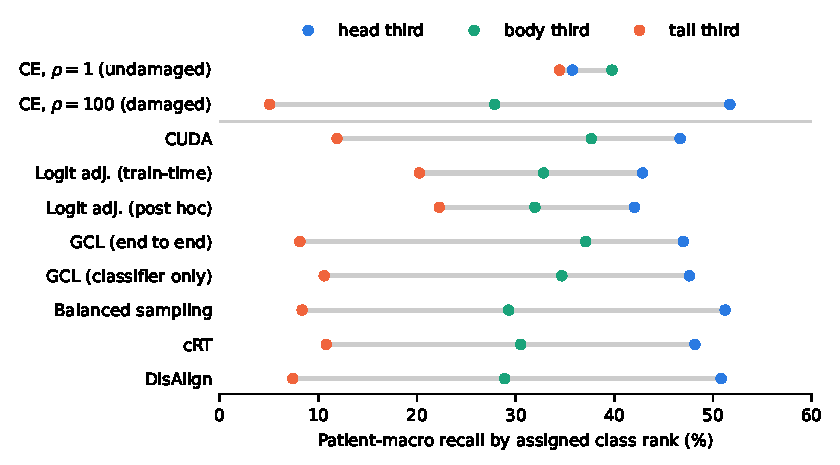
\includegraphics[width=0.78\textwidth]{fig_rank_recall.pdf}
  \caption{Only logit adjustment lifts tail recall substantially at $\rho=100$; CUDA and GCL gain in the body, the other methods stay close to CE. Patient-macro recall of the head, body, and tail thirds of classes by assigned rank, averaged over shards.}
  \label{fig:rank}
\end{figure}

\subsection{Selected strengths}
Validation selection mostly picks interior or theoretically motivated values. At $\rho=100$, logit adjustment selects the full correction $\tau=1$ in 23 of 30 shards in its train-time form, and $\tau=1$ is also the post-hoc mode (15 of 30, with 0.5 in 11). Balanced sampling selects full balancing $s=1$ in 22 of 30. GCL selects $\sigma=0.05$ in 15 (end to end) and 16 (classifier only) of 30, and DisAlign selects $\gamma=1$ or $1.5$ in 22 of 30. CUDA's selected augmentation probability rises with the imbalance: $p_{\mathrm{aug}}=1$ wins 14 of 30 shards at $\rho=100$, 13 of 30 at $\rho=50$, and none at native shares, where 0.25 wins 17. The other selections at $\rho=50$ resemble those at $\rho=100$. At native shares the selections spread across the grid; DisAlign's five values each win between 4 and 8 shards. With no resolved damage, validation accuracy is nearly flat in the strength, and the spread reflects noise rather than a preferred value.

\subsection{Probability quality}
Imbalance mainly worsens raw calibration, and temperature scaling removes most of it for every method. At $\rho=100$ the CE model's raw NLL rises from 2.89 to 3.49 nats and its raw ECE from 28.4 to 36.4 points; even the balanced LoRA model is strongly overconfident. CUDA has by far the lowest raw NLL, 2.25 nats $[2.10, 2.41]$, and raw ECE, 20.8 points $[16.7, 26.4]$, below even the balanced CE model (2.89 and 28.4); the two logit-adjustment forms follow (2.99 and 2.94 nats), and cRT (4.64) and balanced sampling (3.98) are highest. After scaling, every method lies between 1.71 (CUDA) and 1.82 nats, around CE's 1.79 and close to the balanced 1.67, and scaled ECE falls from 12.3 for CE to between 8.8 and 12.3 points. The scaled intervals are unpaired and overlap: CUDA's augmentation curbs raw overconfidence, but no method changes probability quality beyond what temperature scaling already does.

\section{Discussion}
\label{sec:discussion}
\textbf{How much does each method recover?} At $\rho=100$ CUDA gives the most accurate model, recovering about half of the damage against CE, followed by logit adjustment at about two-fifths; six of eight method variants recover a material part. None closes the gap: no paired share interval reaches 1. The ranking is stable from $\rho=50$ to $\rho=100$, and the absolute gains grow with the damage.

\textbf{What do the balanced fits add?} For the quality of the trained classifier, recovery against CE is the relevant reading: it is what a practitioner gains by switching methods on imbalanced data. The balanced fits add how each method behaves without imbalance, and the imbalance-specific recovery follows from that as how much less a method is damaged than CE. The two readings differ only for methods that change accuracy on balanced data, and the difference runs both ways. GCL and cRT make the balanced model slightly worse, cRT by a resolved half point, and are less damaged by the imbalance than their recovery suggests; on this reading classifier-only GCL corrects about half of the damage. The subtraction assumes that the balanced effect carries over unchanged to the imbalanced allocations.

\textbf{Is CUDA's gain an imbalance correction?} Mostly not, but it is still the best classifier. CUDA improves the LoRA model by 1.39 points on the balanced allocation, and this general gain explains its 1.21-point gain at native shares and more than half of its 2.59-point recovery at $\rho=100$. The remaining 1.20 points are not resolved from zero. The point estimate and one descriptive observation leave room for a smaller imbalance-specific part: the selected augmentation probability rises from 0.25 or 0.5 on the balanced allocation to 1 in about half the shards at $\rho=50$ and $\rho=100$. As a correction of imbalance, CUDA's measured contribution is smaller than that of logit adjustment, GCL, and cRT; as a way to train a better LoRA model on BRACS, it is the most effective method tested.

\textbf{Does it matter whether the encoder adapts?} Not for correcting the imbalance. Post-hoc logit adjustment, a fixed prior subtraction at inference, matches every end-to-end method except CUDA, whose recovery exceeds it by 0.65 points in point estimate but whose imbalance-specific part, 1.20 points, falls below it. The largest imbalance-specific correction, 2.41 points, comes from classifier-only GCL, which re-fits only the classifier on a frozen encoder. Without CUDA, the classifier-only family recovers as much as the end-to-end one. Its share under LoRA, about 0.4, exceeds the quarter it recovered under the frozen readout \citep{queisler2026causeBracs}, but the two numbers rest on different damages and classifiers. That the one method acting directly on the class prior is also the only one that restores tail recall fits the large frequency effect found on BRACS under the frozen readout.

\textbf{Does LoRA itself help?} No. LoRA shrinks the measured damage from 7.65 to 4.95 points at $\rho=100$ only because its balanced model is about three points worse than the frozen readout; its imbalanced models are as accurate as the frozen ones. The best mitigated model at $\rho=100$, CUDA at 34.17 percent, stays 5.4 points below the frozen balanced readout. At BRACS's native class shares, LoRA's damage cannot be distinguished from zero and no rebalancing method differs from CE, so in this pipeline rebalancing matters only at severe imbalance; CUDA's gain there matches its gain on the balanced allocation and is a general improvement of the LoRA model.

\textbf{Limitations.} The study covers one dataset, one encoder, and one adaptation scheme. End-to-end training length was tuned on CE at $\rho=100$ only, and a method or allocation that converges more slowly, such as CUDA under strong augmentation, may be disadvantaged at 600 steps. Imbalance-specific recovery assumes that a method's effect on the balanced allocation carries over additively to the imbalanced ones, which the design does not test. The full-recovery reading compares an unpaired interval with a point estimate and is weak whenever the damage is smaller than that interval, as at $\rho=50$; the paired share is the informative reading. The comparison with the frozen readout is descriptive, because the two pipelines differ in classifier and training and share only the test patients.
